\documentclass{article}

\usepackage{fullpage}
\usepackage{graphicx}

\newcommand{\compiler}{DBToaster}
\begin{document}
\title{\compiler\ User Guide}
\author{Yanif Ahmad, Christoph Koch}
\date{\today}
\maketitle

\section{Automated Trading Platform Example}

\begin{figure}[h]
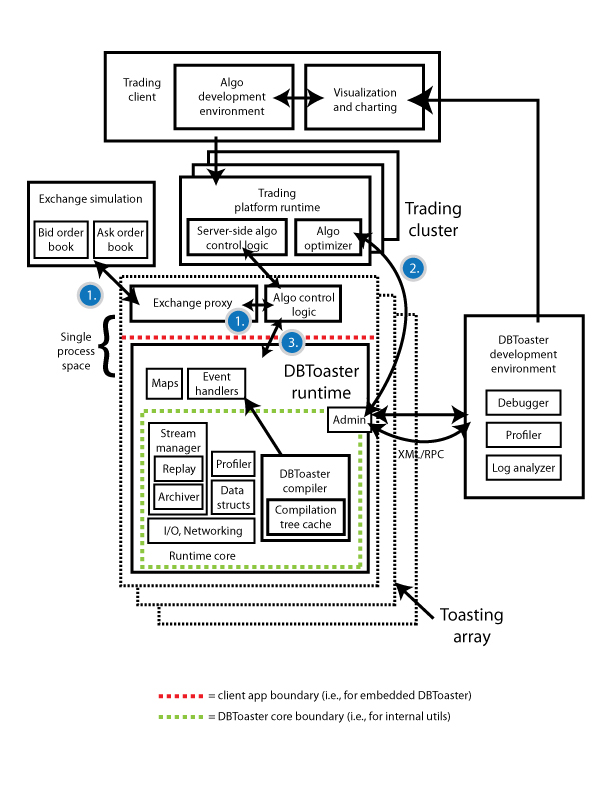
\includegraphics[scale=0.7]{../figures/finapp.jpg}
\label{fig:finapp}
\end{figure}

Key interfaces:
\begin{enumerate}
\item algo$\iff$exchange interface: insert, update, delete order
\begin{verbatim}
	void add_order(bool bid_or_ask, int t, int id, double price, double vol);
	void update_order(bool bid_or_ask, int t, int id, double price, double vol);
	void delete_order(bool bid_or_ask, int id);
\end{verbatim}

\item algo development$\iff$compiler interface: add/remove algo
\begin{verbatim}
	void add_query(string query_id, string query_id,
               string callback_fn = ``void handler(int agg_val) \{\}'');
	void remove_query(string query_id);
\end{verbatim}
 
\item DBToaster$\iff$algo interface: query result callback
\begin{verbatim}
	typedef boost::function<void (int agg_val)> result_callback;
\end{verbatim}
\end{enumerate}

For discussion:
\begin{itemize}
\item what is the user's development/build process?
  \begin{itemize}
  \item e.g., compile DBToaster first, producing \texttt{result\_callback} type,
		and then write client code around the embedded QP.
  \end{itemize}
\end{itemize}

\section{\compiler\ Build Process}
\end{document}
